\documentclass[a4paper]{article}

\usepackage{graphicx}
\usepackage[utf8]{inputenc}
\usepackage[T1]{fontenc}
\usepackage{hyperref}
\usepackage{color}
\usepackage{listings}

% draft watermark
% \usepackage{draftwatermark}
% \SetWatermarkScale{4}

% todo annotations
\usepackage{todonotes}

\addtolength{\textwidth}{3cm}
\addtolength{\oddsidemargin}{-1.5cm}
\addtolength{\evensidemargin}{-1.5cm}
\addtolength{\textheight}{3cm}
\addtolength{\topmargin}{-1.5cm}
\setlength{\parindent}{0pt}
\setlength{\parskip}{1ex}
\pagestyle{plain}

% code listing style
\lstset{
    basicstyle=\footnotesize\ttfamily,
    breaklines=true,
    tabsize=4,
    keepspaces=true,
    columns=flexible,
    % backgroundcolor=\color[gray]{0.9},
    frame=single
}

%%%%%%%%%%%%%%%%%%%%%%%%%%%%%%%%%%%%%%%%%%%%%%%%%%
%% Macros that are filled into the standard text:

%% Things that change for each project:

\newcommand{\Title}{E-Puck2 environment installation}
\newcommand{\Fulltitle}{Installation of the e-puck2 environment}
\newcommand{\Duration}{5-20 min}

\newcommand\tab[1][1cm]{\hspace*{#1}}


%%%%%%%%%%%%%%%%%%%%%%%%%%%%%%%%%%%%%%%%%%%%%%%%%%
%% You won't need to edit anything until the next
%% big remark...

\begin{document}

\raisebox{10mm}{%
 % \footnotesize
  \begin{tabular}{@{\hspace{0pt}}l@{\hspace{0pt}}}
   \textbf{Cours de MICROINFORMATIQUE}\\
   Section de Microtechnique\\
    \raisebox{5mm}{Printemps 2017}\\
    \hline
    \raisebox{-1.2ex}{Practical Exercises}
  \end{tabular}%
}
\hfill

\includegraphics[width=0.3\columnwidth]{fig/logo_epfl_gray.pdf}

\begin{center}
\begin{tabular}{|*{1}{p{0.15\columnwidth}p{0.75\columnwidth}}|}
  \hline
  \multicolumn{2}{|c|}{%
    \raisebox{0pt}[3ex]{\textbf{\Title}}}\\
  \hline
  \raisebox{0pt}[3ex]{\textbf{Title:}}       & \Fulltitle \\
  \raisebox{0pt}[3ex]{\textbf{Duration:}}       & \Duration \\
  \hline
\end{tabular}
\end{center}


%-------------------------------------------------------------------------------
\section{Introduction}
Some programs are needed to program the e-puck2.
\begin{enumerate}
\item Eclipse\_e-puck2 is a distribution of Eclipse IDE for C/C++ Developers specially modified to edit and compile e-puck2's projects out of the box. It doens't require to be installed and everything needed is located in the package given.

The only dependency needed to be able to run Eclipse is Java.
\item Drivers must also be installed for Windows older than Windows 10.

\end{enumerate}

\section{Installation for Windows}


\subsection{Java 32bits}
This section can be ignored if Java 32bits is already installed on your computer.

\begin{enumerate}
\item Go to https://www.java.com/en/download/manual.jsp and download "Windows offline" This is the 32bits version of Java.
\item Run the downloaded installer and follow its intructions to proceed with the installation of Java 32bits.
\item Close the internet browser if it opened at the end of the installation.
\end{enumerate}

\begin{figure}[!h]
\centering
\includegraphics[width=0.5\columnwidth]{fig/Java_Windows}
\caption{Java download page}
\label{fig:Java_windows}
\end{figure}


\subsection{Eclipse\_e-puck2}

\begin{enumerate}
\item Go to the moodle of the course (Microinformatique) and download the Eclipse\_e-puck2 package for windows.
\item Unzip the downloaded file to the location you want (can take time). 

It is strongly recommanded for better performance and less exctraction time to use 7Zip. You can download it on http://www.7-zip.org.
\item You can now run the Eclipse\_e-puck2.exe to launch Eclipse.
\item You can create a shortcut to Eclipse\_e-puck2.exe and place it anywhere if you want.
\end{enumerate}

\begin{figure}[!h]
\centering
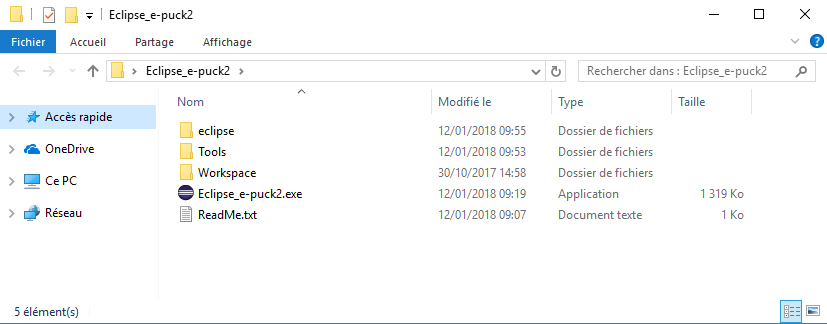
\includegraphics[width=1\columnwidth]{fig/Eclipse_e-puck2_Folder_Windows}
\caption{Eclipse\_e-puck2 folder obtained after extraction}
\label{fig:Eclipse_e-puck2_Folder_Windows}
\end{figure}

\textbf{Important things to avoid :}

\begin{enumerate}
\item The path to the Eclipse\_e-puck2 folder must contain zero space. 

Example :

C:\textbackslash epfl\_stuff\textbackslash Eclipse\_e-puck2   OK

C:\textbackslash epfl stuff\textbackslash Eclipse\_e-puck2   NOT OK
\item The file's structure in the Eclipse\_e-puck2 folder must remains the same. It means no file inside this folder must be moved to another place.
\end{enumerate}

\subsection{Drivers}
This part concerns only the users of a Windows version older than Windows 10. The drivers are automatically installed with Windows 10.

\begin{enumerate}
\item Open zadig-2.3.exe located in the \path{Eclipse_e-puck2\Tools\} you installed before.
\item Connect the e-puck2 with the USB cable and turn it on. Three unknown devices must have appeared in the device list of the program, namely \textbf{e-puck2 STM32F407}, \textbf{e-puck2 GDB Server (Interface 0)} and \textbf{e-puck2 Serial Monitor (Interface 2)}.
\item For each of the three devices mentioned above, select the \textbf{USB Serial (CDC)} driver and click on the "Install Driver" button to install it. Accept the different prompts which may appear during the process. After that you can simply quit the program and the drivers are installed. These steps are illustrated on Figure \ref{fig:Zadig_e-puck2_STM32F407} below.

Note : The drivers installed are located in \path{C:\Users\"your_user_name"\usb_driver}
\end{enumerate}

\begin{figure}[!h]
\centering
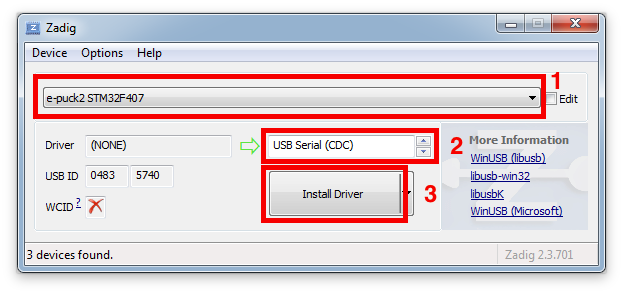
\includegraphics[width=0.7\columnwidth]{fig/Zadig_e-puck2_STM32F407}
\caption{Example of driver installation for \textbf{e-puck2 STM32F407}}
\label{fig:Zadig_e-puck2_STM32F407}
\end{figure}

\newpage
\section{Installation for Linux}

\subsection{Java}
This section can be ignored if Java is already installed on your computer.

\begin{enumerate}
\item Type the following commands in a terminal session to install Java SDK
\begin{lstlisting}
$ sudo add-apt-repository ppa:openjdk-r/ppa
$ sudo apt-get update
$ sudo apt-get install openjdk-8-jre
\end{lstlisting}
\end{enumerate}


\subsection{Eclipse\_e-puck2}

\begin{enumerate}
\item Go to the moodle of the course (Microinformatique) and download the Eclipse\_e-puck2 package for Linux.
Pay attention to the 32bits or 64bits version.
\item Extract the downloaded file to the location you want (can take time). 
\item You can now run the Eclipse\_e-puck2 executable to launch Eclipse.
\end{enumerate}

\begin{figure}[!h]
\centering
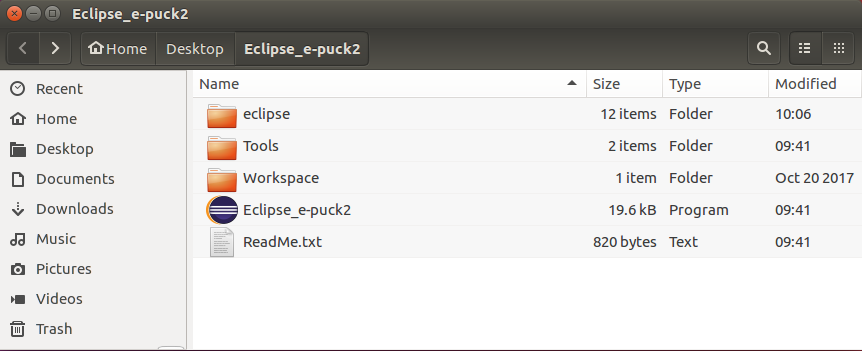
\includegraphics[width=1\columnwidth]{fig/Eclipse_e-puck2_Folder_Linux}
\caption{Eclipse\_e-puck2 folder obtained after extraction}
\label{fig:Eclipse_e-puck2_Folder_Linux}
\end{figure}

Note : The icon of the Eclipse\_e-puck2 executable will appear after the first launch of the program.

\textbf{Important things to avoid :}

\begin{enumerate}
\item You can not create a Link to the Eclipse\_e-puck2 executable because otherwise the program will think its location is where the Link is and it will not find the ressources located in the Eclipse\_e-puck2 folder.
\item The path to the Eclipse\_e-puck2 folder must contain zero space. 

Example :

/home/student/epfl\_stuff/Eclipse\_e-puck2 OK   OK

/home/student/epfl stuff/Eclipse\_e-puck2 NOT OK

\item The file's structure in the Eclipse\_e-puck2 folder must remains the same. It means no file inside this folder must be moved to another place.
\end{enumerate}

\subsection{Serial Port}

In order to let Eclipse, or any program ran by you to access the serial ports, a little configuration is needed.

Type the following command in a terminal session. Once done, you need to log off to let the change take effect.

\begin{lstlisting}
$ sudo adduser $USER dialout
\end{lstlisting}

\newpage
\section{Installation for Mac}

\subsection{Java}
This section can be ignored if Java is already installed on your computer.

\begin{enumerate}
\item Go to http://www.oracle.com/technetwork/java/javase/downloads/jdk8-downloads-2133151.html and download the Mac OS X Java 8 SE Development Kit. It is the .dgm file \textbf{without} the Demos and Samples.
For example : jdk-8uXXX-macosx-x64.dmg
\item Open the .dmg file downloaded, run the installer and follow the instructions to proceed with the installation of Java SDK.
\end{enumerate}

\begin{figure}[!h]
\centering
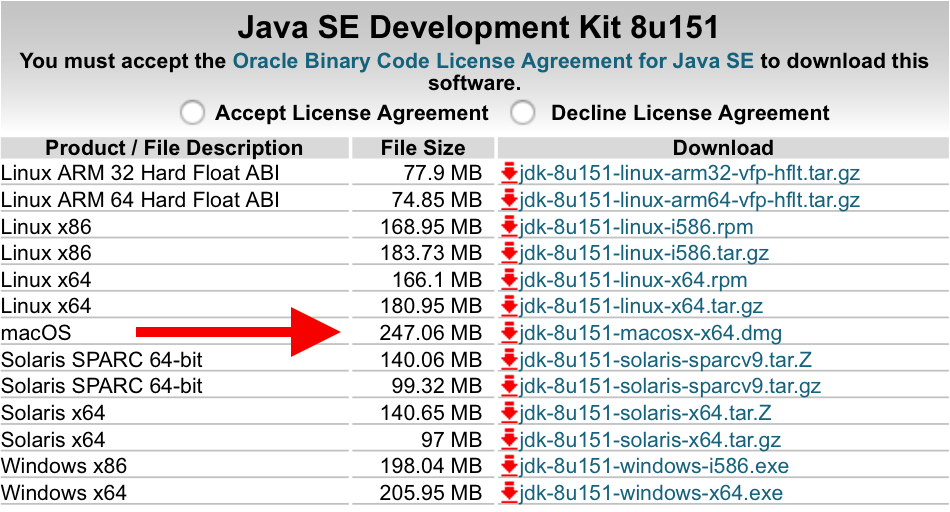
\includegraphics[width=0.7\columnwidth]{fig/Java_mac}
\caption{Java download page}
\label{fig:Java_mac}
\end{figure}

\subsection{Eclipse\_e-puck2}

\begin{enumerate}
\item Go to the moodle of the course (Microinformatique) and download the Eclipse\_e-puck2 package for Mac.
\item Open the .dmg file downloaded and DragAndDrop the Eclipse\_e-puck2.app into the Applications folder

Note : You can place the Eclipse\_e-puck2.app anywhere, as long a the full path to it doesn't contain any space, if you don't want it to be in Applications.
\item You can create an Alias to Eclipse\_e-puck2.app and place it anywhere if you want.
\end{enumerate}

\subsection{First launch and Gatekeeper}

It's very likely that Gatekeeper (one of the protectons of Mac OS) will prevent you to launch Eclipse\_e-puck2.app because it isn't signed from a known developper. 

If you can't run the program because of a warning of the system. Press OK and try to launch it by right clicking on it and choosing "open" in the contextual menu (may be slow to open the first time).

If « Unable to open "Eclipse\_e-puck2.app" because this app comes from an unidentified developer. »  

or if « "Eclipse.app" is corrupted and can not be opened. You should place this item in the Trash. »

appears after executing the app the first time, it is needed to disable temporarily Gatekeeper.

To do so :
\begin{enumerate}
\item Go to System Preferences->security and privacy->General and authorize downloaded application from \textbf{Anywhere}.

If you are on Mac OS Sierra or greater (greater or equal to Mac OS 10.12), you must type the following command on the terminal to make the option above appear.
\begin{lstlisting}
$ sudo spctl --master-disable
\end{lstlisting}
\item Now you can try to run the application and it should work.
\item If Eclipse opened successfully, it is time to reactivate Gatekeeper. Simply set back the setting of gatekeeper.

For the ones who needed to type a command to disable Gatekeeper, her is the command to reactivate it.
\begin{lstlisting}
sudo spctl --master-enable
\end{lstlisting}
\end{enumerate}

\begin{figure}[!h]
\centering
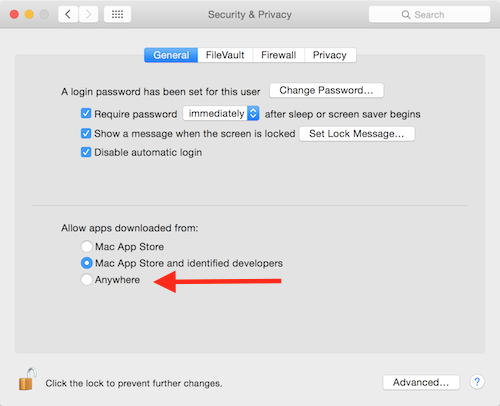
\includegraphics[width=0.7\columnwidth]{fig/security_tab_mac}
\caption{Security settings of Mac OS}
\label{fig:security_tab_mac}
\end{figure}

This procedure is only needed the first time. After that Gatekeeper will remember your choice to let run this application and will not bother you anymore, as long as you use this application. If you re-download it, you will have to redo the procedure for Gatekeeper.



\textbf{Important things to avoid :}

\begin{enumerate}
\item The path to the Eclipse\_e-puck2.app must contain zero space. 

Example :

/home/student/epfl\_stuff/Eclipse\_e-puck2 OK   OK

/home/student/epfl stuff/Eclipse\_e-puck2 NOT OK

\item The file's structure in the Eclipse\_e-puck2.app must remains the same. It means no file inside this app must be moved to another place.
\end{enumerate}

\end{document}
